\chapter{Methodology \& Technology}

\begin{FraseCelebre}
  \begin{Frase}
    The needs of the many outweigh the needs of the few
  \end{Frase}
  \begin{Fuente}
    Spock - The Wrath of Khan
  \end{Fuente}
\end{FraseCelebre}

\section{Methodology}
The idea of this project came up in a Hackathon in September 2017. We were a
group of 4 developers and we had one month to create an idea and a small
prototype to implement in the blockchain.

To give birth to the idea of a decentralized publication system for open science
we used agile methodologies.


\subsection{Brainstorming}

Brainstorming was part of the first step to define what are we going to do. We
throwed a lot of ideas into a white board without discrimination, no matter if
the ideas were very hard or easy to implement.


After saying enough ideas to fill the board we filtered the ones that were
impossible to achieve. Then, each one voted the best three, making a ranking of
the 3-4 best projects to start working on. Finally, we argued what were the best
one and then we started developing the project backbone.


After the first session of brainstorming that lasted approximately 4 hours we
were ready to create a value proposition canvas to define all the aspects of the
project.

\subsection{Value proposition canvas}


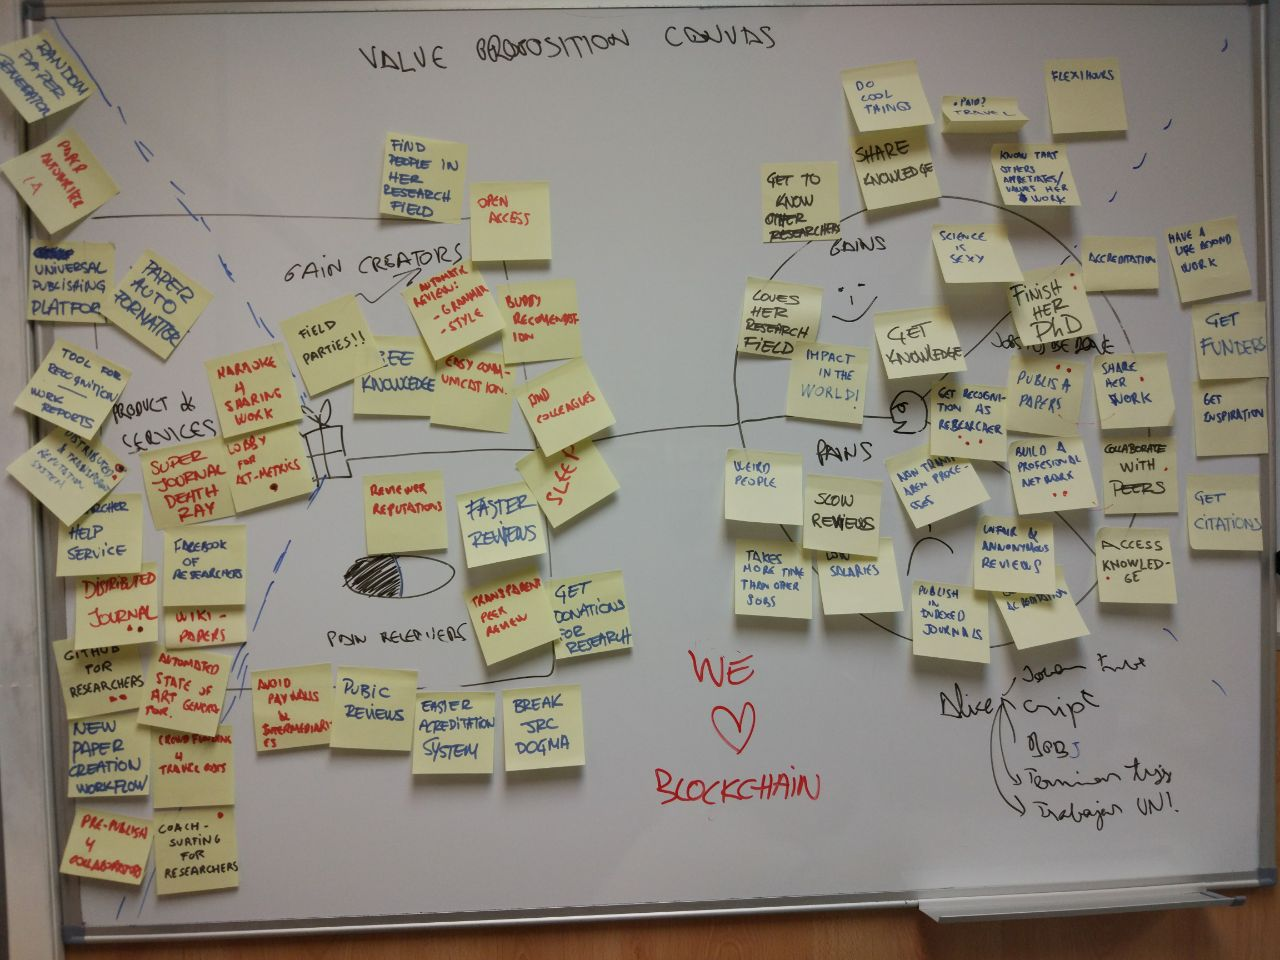
\includegraphics[width=0.9\linewidth]{Imagenes/vpc.jpg}

\section{Technology}

To face the challenges proposed by this project, there are many possibilities to
distribute both the data and the information about the reputation network. To
build a robust and decentralized system i

% -------------------------------------------------------------------
\subsection{IPFS}
% -------------------------------------------------------------------
\label{tech:sec:ipfs}
IPFS stands for Interplanetary File System. It is a peer-to-peer file-sharing
protocol that uses a cryptographic hashes to store files in a distributed
network. IPFS works very similar to HTTP protocol but in a BitTorrent way. It
can be seen as a giant git repository where everyone can store, share and
exchange files\cite{benet2014ipfs}.

IPFS merges three main ideas: Distributed Hash Tables, BitTorrent, Git and
Self-Certified Systems.

\subsubsection{Distributed Hash Tables}
A distributed hash table(\emph{DHT}) is a decentralized structure that works
very similar to a hash table. Hash tables are used to identify items in a
database. The table performs simple mathematical operations generating a random
string called hash. The hash acts as a pointer that directs to the data, this
allows the user to find data directly instead of looking through the entire
database\cite{kaluszka2010distributed}.

In a distributed hash table, any node can use a hash as a key to retrieve data.
This system includes a data structure called ``keyspace'' that is a set of all
possible keys, which is split up across the nodes in the system. The mapping of
the keys is made by another function that describes the distance from one key to
another. All the nodes have and identifier and a set of identifiers pointing to
all its neighbors nodes. If a node is removed from the network, only a small
portion of the data must be recovered by other
nodes\cite{kaluszka2010distributed}.

This system makes \emph{DHTs} scalable, fast and robust. It is used by
frameworks such as Tapestry \cite{zhao2004tapestry}, Chord
\cite{stoica2001chord}, Kelips \cite{gupta2003kelips}, Kademlia
\cite{maymounkov2002kademlia} and IPFS \cite{benet2014ipfs}. These platforms are
similar in cost and performance if they are tested in a large enough network.
They behave very fast when it comes to searching for a key through massive
networks of nodes\cite{li2004comparing}, that's why it is used by IPFS to create
its distributed file system.

\subsubsection{BitTorrent - File sharing}
BitTorrent \cite{cohen2003incentives} is a P2P file sharing system used
worldwide. In this system, files are divides into very small chucks of data, and
are shared in a peer-to-peer network. Each peer aims to maximize its download
rate by connecting to low latency peers. In BitTorrent's network, peers with
high upload rate will get higher download rate, so the key is balancing the
network bandwidth between downloading and uploading
files\cite{pouwelse2005bittorrent}.

IPFS uses three main features from BitTorrent's protocol\cite{benet2014ipfs}:
\begin{itemize}
\item BitTorrent's data exchange protocol rewards nodes who contribute to the
  network, and punishes the ones who don't.
\item BitTorrent tracks the availability of file chunks, sending the rarest
  first rather than sending the most common ones.
\item IPFS uses PropShare\cite{levin2008bittorrent} bandwidth allocation
  strategy to improve BitTorrent's behavior facing exploitable scenarios.
\end{itemize}

\subsubsection{Git - Version control system}
Git is a distributed version control system (\emph{DVCS})\cite{torvalds2010git}.
Git was born in 2005 when the development process of the Linux kernel lost its
version control system. The Linux kernel is one of the biggest free software
projects nowadays, it has a great team of developers behind and the code usually
changes very frequently. In 2002 the team used BitKeeper as VCS since they had a
free license. But in 2005 when this license was over, Linus Torvalds decided to
develop his own VCS\cite{spinellis2005version}.

Git was designed to be scalable and distributed, and the most important factors
that IPFS inherits from Git are: \cite{benet2014ipfs}:

\begin{itemize}
\item Git implements a Merkle Directed Acyclic Graph
  \cite{bleichenbacher1994directed}, an object that reflects changes in a file
  system in a distributed way.
\item Objects are identified by the cryptographic hash of their contents.
\item Version changes only update preferences and add objects. To broadcast
  version changes, git only needs to transfer the new objects and update the
  remote references.
\end{itemize}

\subsubsection{Self-Certified File Systems}




%%% Local Variables:
%%% mode: latex
%%% TeX-master: "../Tesis.tex"
%%% End:
